\chapter{Arhitektura i dizajn sustava}

		Na najvišoj razini apstrakcije naš sustav podijeljen je na klijenta i poslužitelja koji komunicira s bazom podataka.
		
		Pomoću web preglednika korisnik se povezuje na web stranicu preko HTTP-a na kojoj interagira s klijentskim dijelom sustava, dakle korisničkim sučeljem. Zahtjevi koje šalje korisnik obrađuje poslužitelj koji po potrebi sprema i preuzima podatke iz baze te vraća korisniku preko klijenta povratnu informaciju.
	
		Arhitektura sustava našeg programskog rješenja dizajnirana je suvremenim pristupom, rabeći Model-View-Controller (MVC) paradigmu koja osigurava smislenu podjelu sustava na manje cjeline prema funkcionalnosti i povezuje backend pisan u C\#-u uz ASP.NET radni okvir, frontend razvijen u htmx-u i JavaScriptu i bazu podataka ostvarenu PostgreSQL-om.


		\begin{itemize}
			\item \textbf{Model:} Mozak sustava, zadužen je za procesuiranje, spremanje i obradu podataka, izvođenje funkcija i općenitog rada sustava. 
			\item \textbf{Controller:} Poput mosta, povezuje sustav s korisničkim unosima. Provodi preliminarnu obradu zahtjeva i prosljeđuje ih modelu i pogledu.
			\item \textbf{View:} Sadrži stvari koje se prikazuju korisniku preko sučelja aplikacije te površinske funkcionalnosti interakcije s korisnikom i promjena prikaza.
		\end{itemize}
		
		\subsection*{Radni tijek}
		
		\begin{itemize}
			\item Korisnik rabi web aplikaciju preko sučelja, šaljući zahtjeve poput unosa teksta u tražilicu.
			\item Kontroler prima zahtjeve, obrađuje ih i prenosi ih modelu.
			\item Model prema potrebi komunicira s bazom podataka, dohvaća potrebne podatke i ispunjava zahtjev.
			\item Kontroler prima procesuirane podatke od modela i prosljeđuje ih pogledu gdje se podaci dinamički predstavljaju korisniku.
		\end{itemize}
				
		\section{Baza podataka}
		
		
		Za potrebe naše aplikacije koristimo relacijsku bazu podataka kako bismo lakše spremili i dohvaćali potrebne podatke. Baza se temelji na relacijama, tj. na tablicama definiranim imenom i atributima.
		
		\subsection{Opis tablica}
		
		Ova tablica sadrži sve potrebne informacije o korisniku, kao što su:
		korisničko ime, lozinku korisnika, korisnikovo ime i prezime, koja je vrsta korisnika, njegov e-mail, broj mobitela, stanje odobrenosti, adresu, grad, koordinate i državu u kojoj se nalazi. Ona je u "One-to-Many" vezi s tablicom Knjiga preko svojeg ID-a.
		\begin{longtblr}[
			label=none,
			entry=none
			]{
				width = \textwidth,
				colspec={|X[6,l]|X[6, l]|X[20, l]|}, 
				rowhead = 1,
			} %definicija širine tablice, širine stupaca, poravnanje i broja redaka naslova tablice
			\hline \SetCell[c=3]{c}{\textbf{Korisnik}}	 \\ \hline[3pt]
			\SetCell{LightGreen}ID ponuditelj & INT	&  Jedinstveni identifikator korisnika u tablici	\\ \hline
			korisnicko ime	& VARCHAR & korisničko ime izdavača, antikvarijata ili preprodavača  	\\ \hline 
			lozinka & VARCHAR & lozinka korisnika  \\ \hline 
			naziv korisnika & VARCHAR	& ime i prezime korisnika 		\\ \hline 
			vrsta korisnika & VARCHAR	& korisnik može biti izdavač, antikvarijat ili preprodavač 		\\ \hline 
			email & VARCHAR	& e-mail korisnika		\\ \hline 
			broj mobitela & INT	& korisnikov broj mobitela		\\ \hline 
			adresa & VARCHAR	& adresa korisnika 		\\ \hline 
			odobren & BOOLEAN	& govori nam je li korisnik odobren (registriran) u sustavu, tj. može li se prijaviti		\\ \hline 
			drzava & VARCHAR	& država u kojoj se nalazi korisnik 		\\ \hline 
			grad & VARCHAR	& grad u kojem se nalazi korisnik 		\\ \hline 
			koordinate & FLOAT	& geografske koordinate korisnika		\\ \hline 
			
			
		\end{longtblr}
		Ova tablica sadrži sve potrebne informacije o knjigama, kao što su:
		naziv, ime i prezime autora, godina izdanja, naziv i vrstu izdavača, ISBN, broj
		izdanja, opis knjige, jezik na kojem je izdan i dostupnost. Ona je u
		One-to-One vezi s tablicom Korica preko svojeg ID-a, u "Many-To-One" vezi s tablicom Korisnik preko njezinog ID-a i u "One-to-Many" vezi s tablicom Ponuda preko svojeg ID-a.
		
		
		\begin{longtblr}[
			label=none,
			entry=none
			]{
				width = \textwidth,
				colspec={|X[6,l]|X[6, l]|X[20, l]|}, 
				rowhead = 1,
			} %definicija širine tablice, širine stupaca, poravnanje i broja redaka naslova tablice
			\hline \SetCell[c=3]{c}{\textbf{Knjiga}}	 \\ \hline[3pt]
			\SetCell{LightGreen}ID naslov & INT	&  Jedinstveni identifikator knjige u tablici	\\ \hline
			naziv	& VARCHAR & naziv knjige   	\\ \hline 
			autor & VARCHAR & ime i prezime autora  \\ \hline 
			godina izdavanja & INT	& godina u kojoj je izdana knjiga 		\\ \hline 
			izdavac & VARCHAR	& naziv izdavača knjige 		\\ \hline 
			kategorija izdavaca & VARCHAR	& vrsta izdavača (domaći ili strani)		\\ \hline 
			zanr & VARCHAR	& žanr knjige		\\ \hline 
			ISBN & INT	& međunarodni identificator knjiga 		\\ \hline 
			broj izdanja & INT	& broj trenutnog izdanja knjige	\\ \hline 
			opis & VARCHAR	& kratki opis o radnji knjige		\\ \hline
			jezik & VARCHAR	& jezik na kojem je izdana knjiga 		\\ \hline
			dostupnost & VARCHAR & trenutna dostupnost knjige \\ \hline
			\SetCell{LightBlue} ID ponuditelj	& INT &  Identifikator korisnika iz tablice Korisnik 	\\ \hline 
			
			
		\end{longtblr}
		
		
		
		Ova tablica sadrži sve potrebne informacije o dostupnim ponudama, kao što su:
		cijena knjige i broj dostupnih knjiga. Ona je u
		u "Many-to-One" vezi s tablicom Knjiga preko njezinog ID-a.
		\begin{longtblr}[
			label=none,
			entry=none
			]{
				width = \textwidth,
				colspec={|X[6,l]|X[6, l]|X[20, l]|}, 
				rowhead = 1,
			} %definicija širine tablice, širine stupaca, poravnanje i broja redaka naslova tablice
			\hline \SetCell[c=3]{c}{\textbf{Ponuda}}	 \\ \hline[3pt]
			\SetCell{LightGreen}ID & INT	&  Jedinstveni identifikator ponude u tablici	\\ \hline
			cijena	& FLOAT & cijena u eurima po kojoj se knjiga nudi	\\ \hline
			stanje & VARCHAR	& trenutno stanje očuvanosti knjige \\ \hline 
			broj primjeraka	& INT & trenutni broj dostupnih knjiga	\\ \hline 
			\SetCell{LightBlue} ID knjige	& INT &  Identifikator knjige iz tablice Knjiga  	\\ \hline 
			
		\end{longtblr}
		Ova tablica sadrži slike korica knjiga. Ona je u 
		"One-to-One" vezi s tablicom Knjiga ID-a od knjige.
		\begin{longtblr}[
			label=none,
			entry=none
			]{
				width = \textwidth,
				colspec={|X[6,l]|X[6, l]|X[20, l]|}, 
				rowhead = 1,
			} %definicija širine tablice, širine stupaca, poravnanje i broja redaka naslova tablice
			\hline \SetCell[c=3]{c}{\textbf{Korica}}	 \\ \hline[3pt]
			\SetCell{LightGreen}ID & INT	&  Jedinstveni identifikator korice u tablici	\\ \hline
			slika	& BLOB & Slika korice (spremljeno u bazi u BLOB formatu)	\\ \hline
			tip slike & VARCHAR & Sadrži vrstu slike (npr. "image/jpg")\\ \hline 
			\SetCell{LightBlue} ID naslov	& INT &  Identifikator knjige iz tablice Knjiga  	\\ \hline 
			
		\end{longtblr}
		
		
		
		\subsection{Dijagram baze podataka}
		
		\begin{figure}[hbt!]
			\centering
			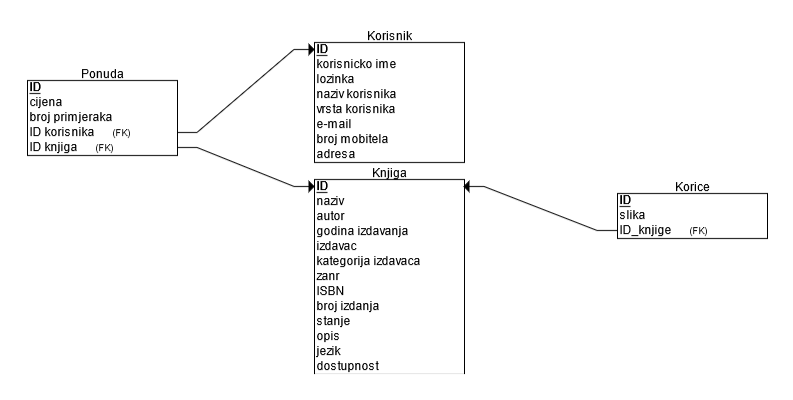
\includegraphics[width = \textwidth]{slike/Relacijska shema}
			\caption{Slika relacijske sheme}
			\label{fig:enter-label}
		\end{figure}
		
		\eject
			
		\section{Dijagram razreda}
		
			Paket \textit{Model} preslikava bazu podataka u aplikaciji. Razred \textit{Book} predstavlja knjigu koja je objavljena na stranici. Razred \textit{BookCover} predstavlja naslovnicu knjige. Razred \textit{Offer} predstavlja ponudu za neku knjigu. Razred \textit{User} predstavlja registriranog korisnika koji može stvarati nove objave na stranici. Razredi \textit{UserType}, \textit{PublisherType}, \textit{Language}, \textit{Country} sadrže vrste atributa korisnika te njihovi atributi imaju predodređene vrijednosti. Razred \textit{RegisterRequest} služi za dodavanje novog korisnika.\\
				
			Paket \textit{Controller} sadrži klase \textit{NpgsqlRepository}, \textit{AccountController}, \textit{HomeController} i \textit{BookController}. U razredu \textit{AccountController} nalaze se sve metode potrebne za prijavu ili registraciju korisnika. U klasi \textit{HomeController} nalaze se metode potrebne za korištenje web-aplikacije. Razred \textit{BookController} sadrži metode za upravljanje knjigama i njihovim ponudama. U razredu \textit{NpgsqlRepository} nalaze se metode potrebne za upravljanje knjigama, korisnicima i prijevodima, npr. brisanje, dodavanje, ažuriranje ili dohvat.\\
			
			\clearpage
			
			\begin{figure}[h]
				\centering
				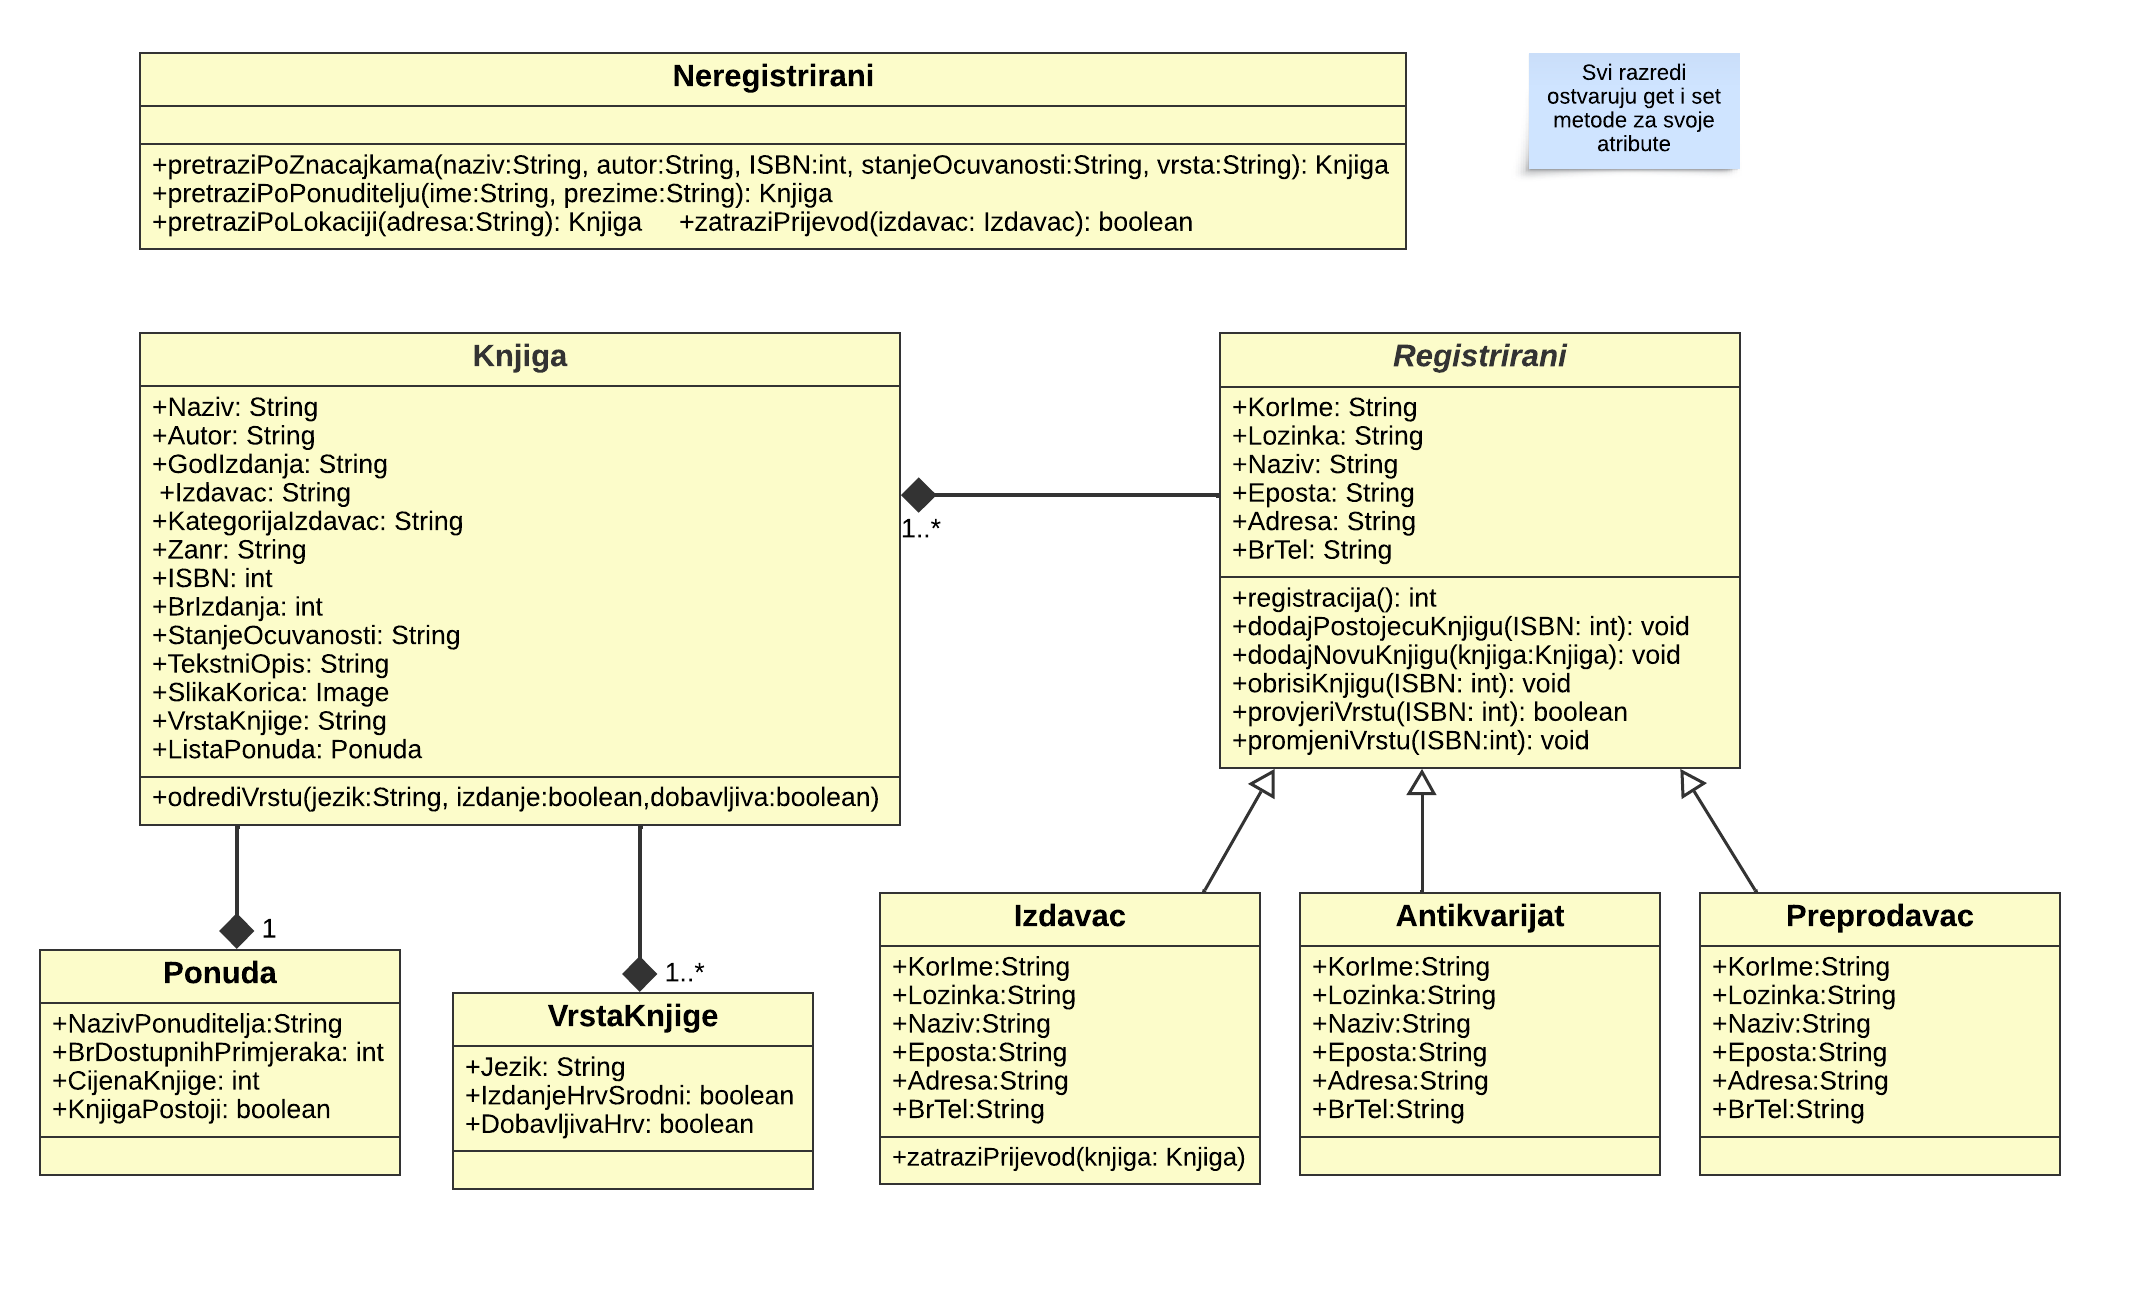
\includegraphics[width = \textwidth]{slike/dijagramKlasa.PNG}
				\caption{Dijagram razreda}
				\label{fig:enter-label}
			\end{figure}
			
			\clearpage
		
		\section{Dijagram stanja}
			
			
			Dijagram stanja objašnjava stanja u kojima se web stranica može nalaziti i kako se prelazi iz jednog stanja u drugo.\\
			Na slici se prikazuju stanja i prijelazi za registriranog korisnika. Za neregistriranog je uglavnom isto, samo što se mogu registrirati i prijavit, ali  ne mogu pregledavati svoj račun.\\
			Sa glavne stranice korisnik može: pregledati svoj račun i od tamo pregledavati, dodavati i brisati objave, otići na traženje i filtriranje knjiga i odjaviti se iz svog računa.\\
			Kod tražilice se može otići na objavu, a kod objave na profil ponuditelja i obrnuto. \\
			U bilo kojem trenutku se može doći na početnu stranicu, stranicu za traženje i filtriranje i u bilo kojem trenutku je moguće napraviti registraciju, prijavu i odjavu.

           		\begin{figure}[h]
				\centering
				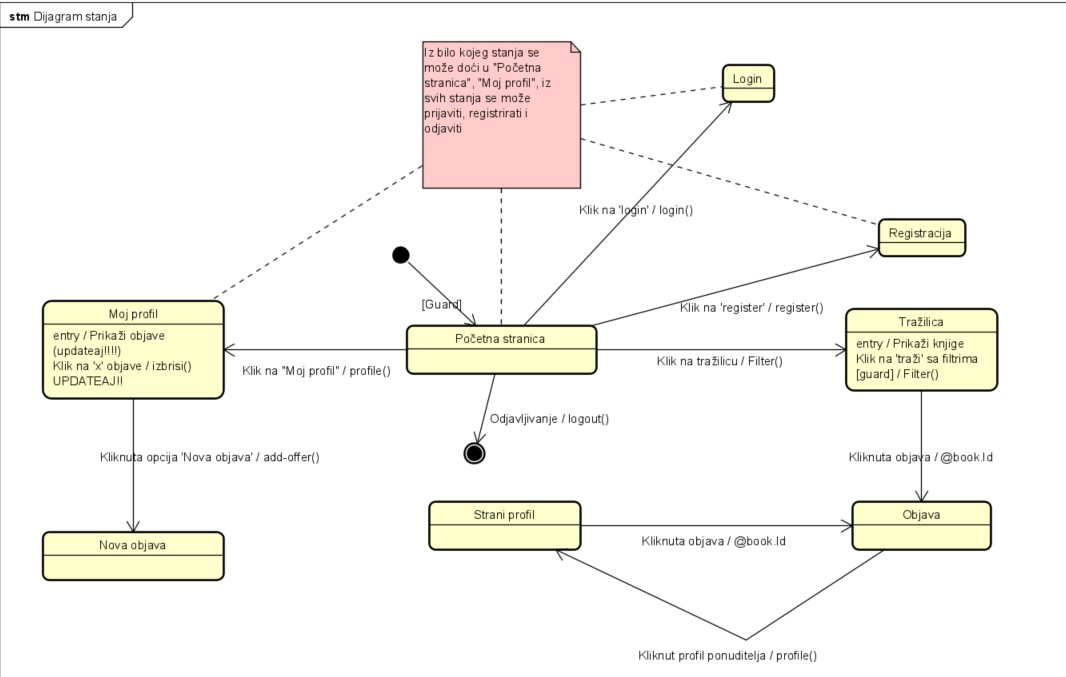
\includegraphics[width = \textwidth]{slike/dijagram_stanja.jpg}
				\caption{Dijagram aktivnosti dodavanja nove objave knjige}
				\label{fig:enter-label}
			\end{figure}
			
			\eject 
			
		
		\section{Dijagram aktivnosti}
		
			\raggedright{Dijagram aktivnosti prikazuje proces dodavanja nove objave za korisnika koji je već registriran. Prva stvar koju mora napraviti jest prijava u sustav. Nakon toga pomoću opcije Nova objava dodaje ono što želi. Objava se sprema u bazu podataka i postaje vidljiva na stranici.}\\
			
			\begin{figure}[h]
				\centering
				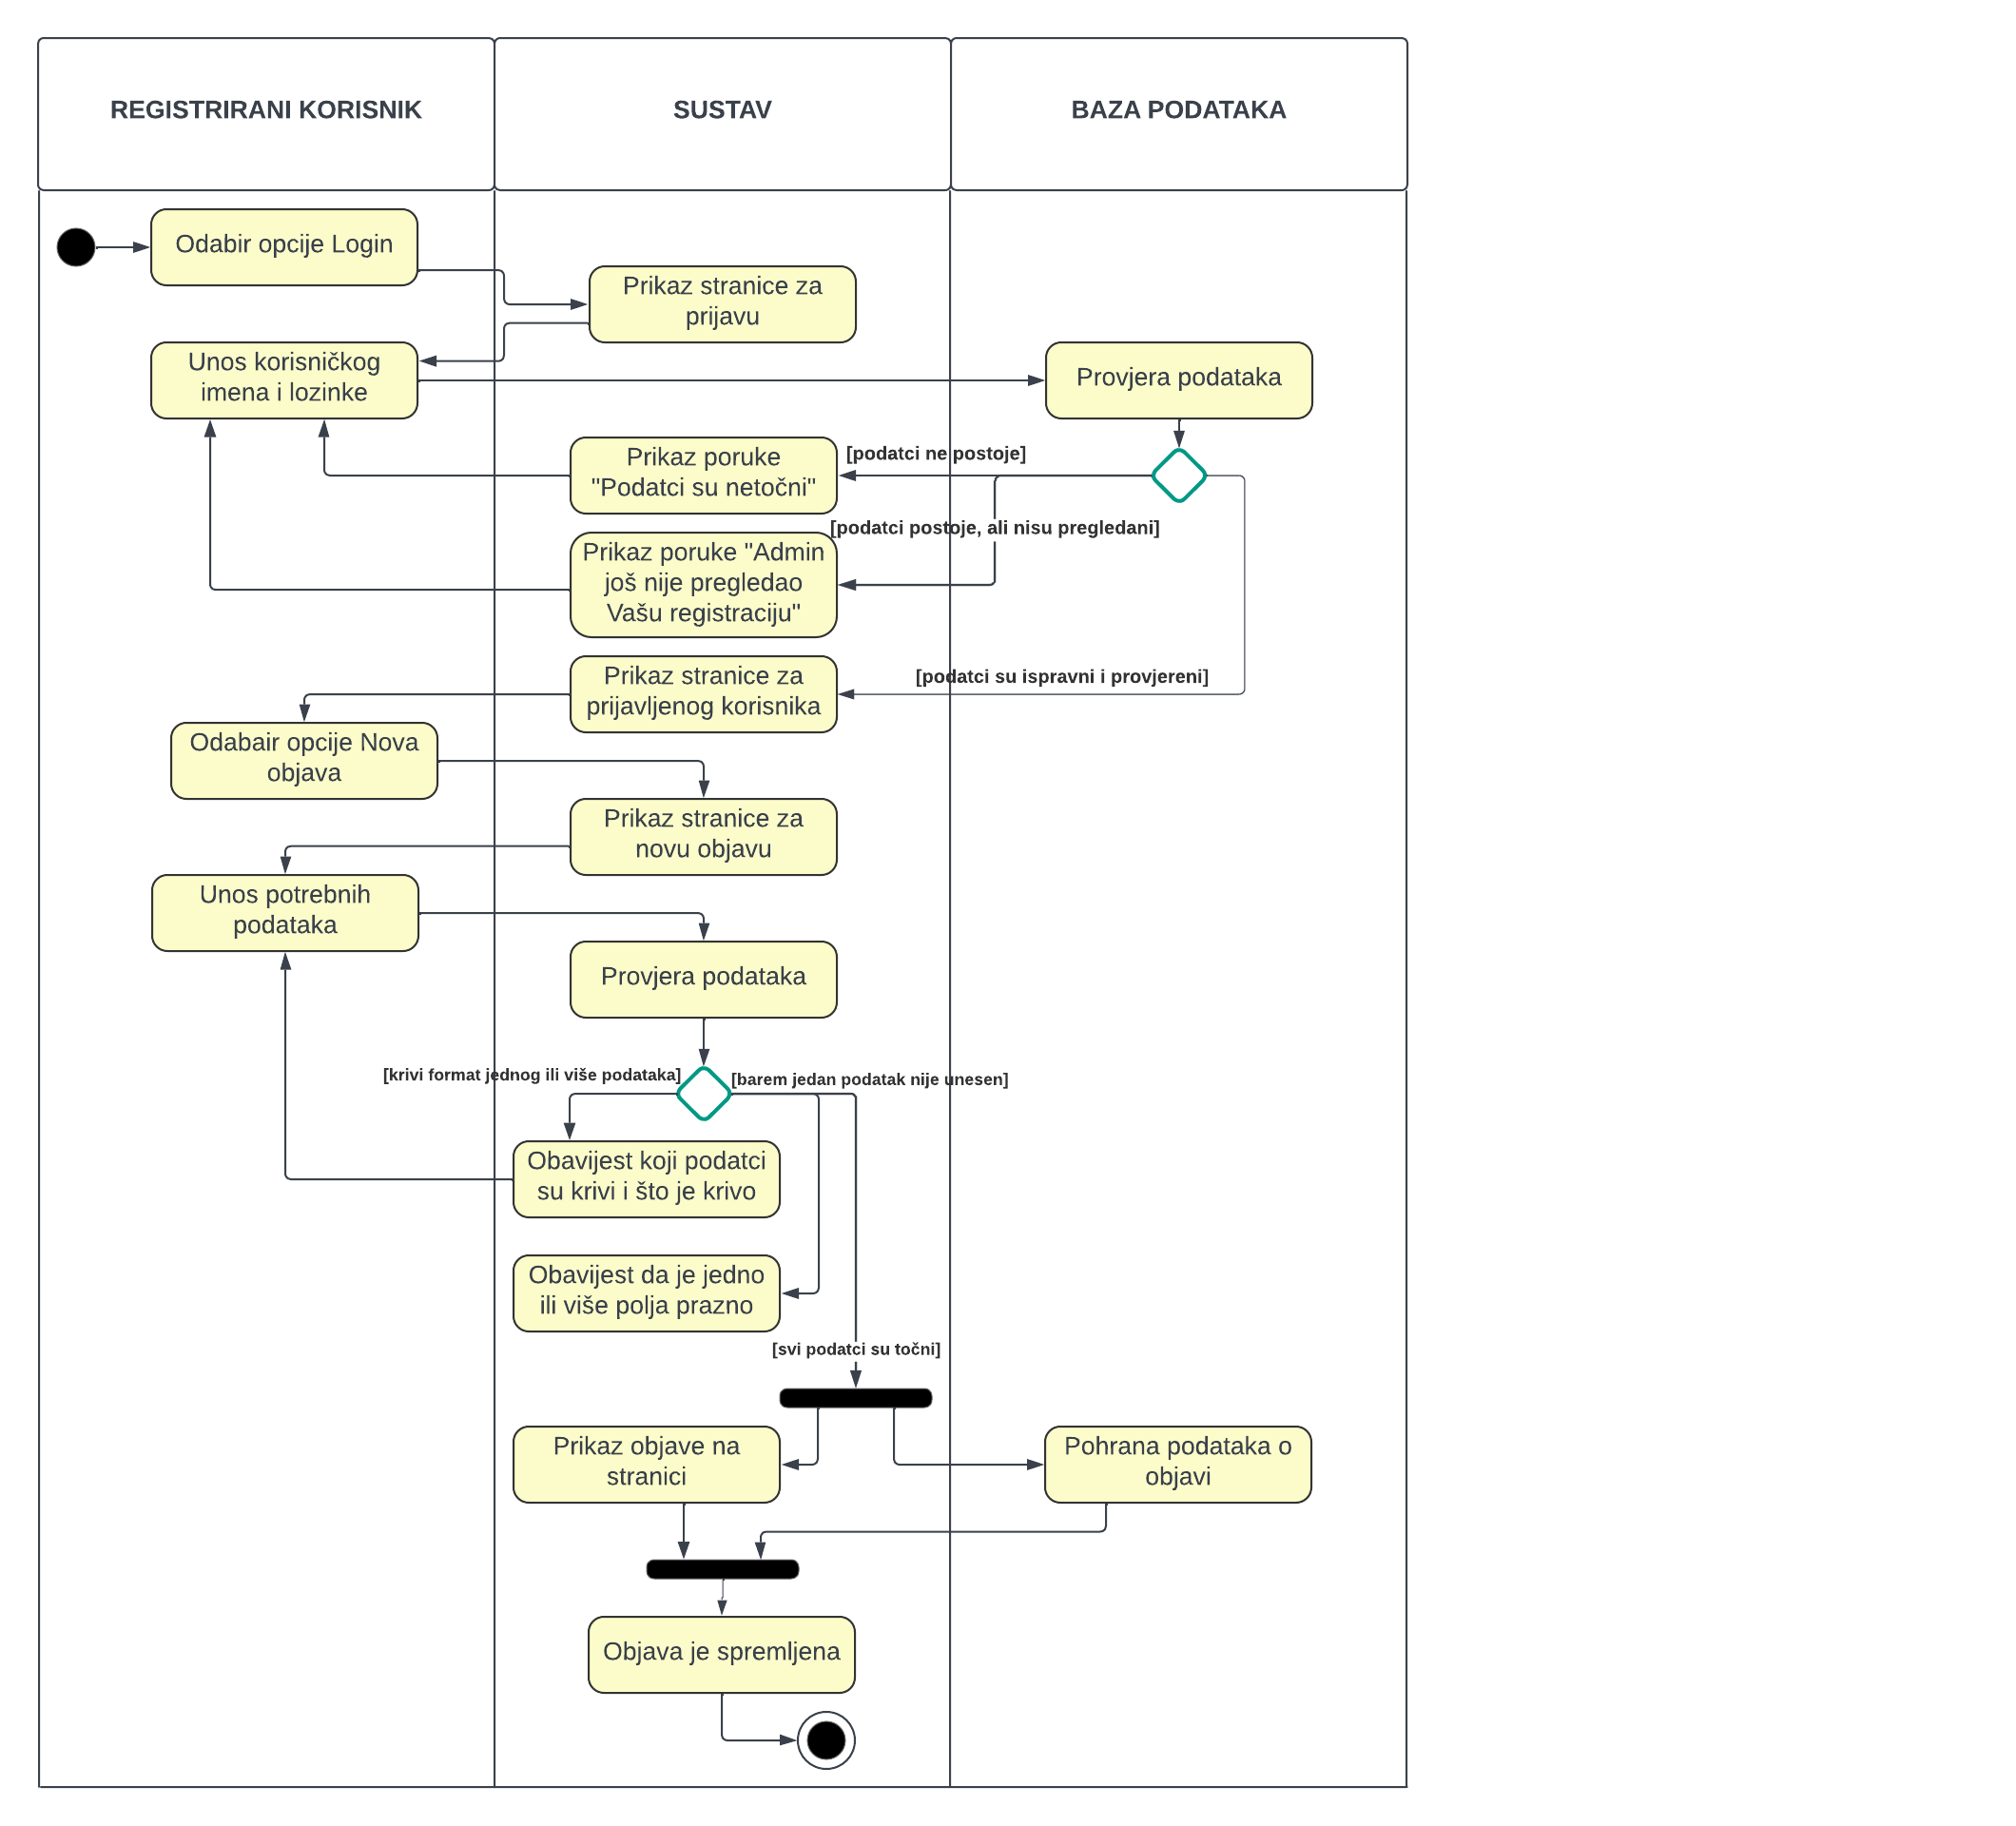
\includegraphics[width = \textwidth]{slike/dijagram_akt.PNG}
				\caption{Dijagram aktivnosti dodavanja nove objave knjige}
				\label{fig:enter-label}
			\end{figure}
			\eject
			
		\section{Dijagram komponenti}
		
			\raggedright{Dijagram komponenti prikazuje strukturu cijele aplikacije. Web-aplikacija sastoji se od 6 komponenti: Controllers, Helpers, Models, Misc, Dto i Views. Controllers pružaju REST\_API sučelje na koje vanjski web-preglednik može slati zahtjeve. Controllers koriste SQL kako bi pristupili bazi podataka. Za pretvorbu podataka iz Modela u html koristi se Razor.}\\
			
			\begin{figure}[h]
				\centering
				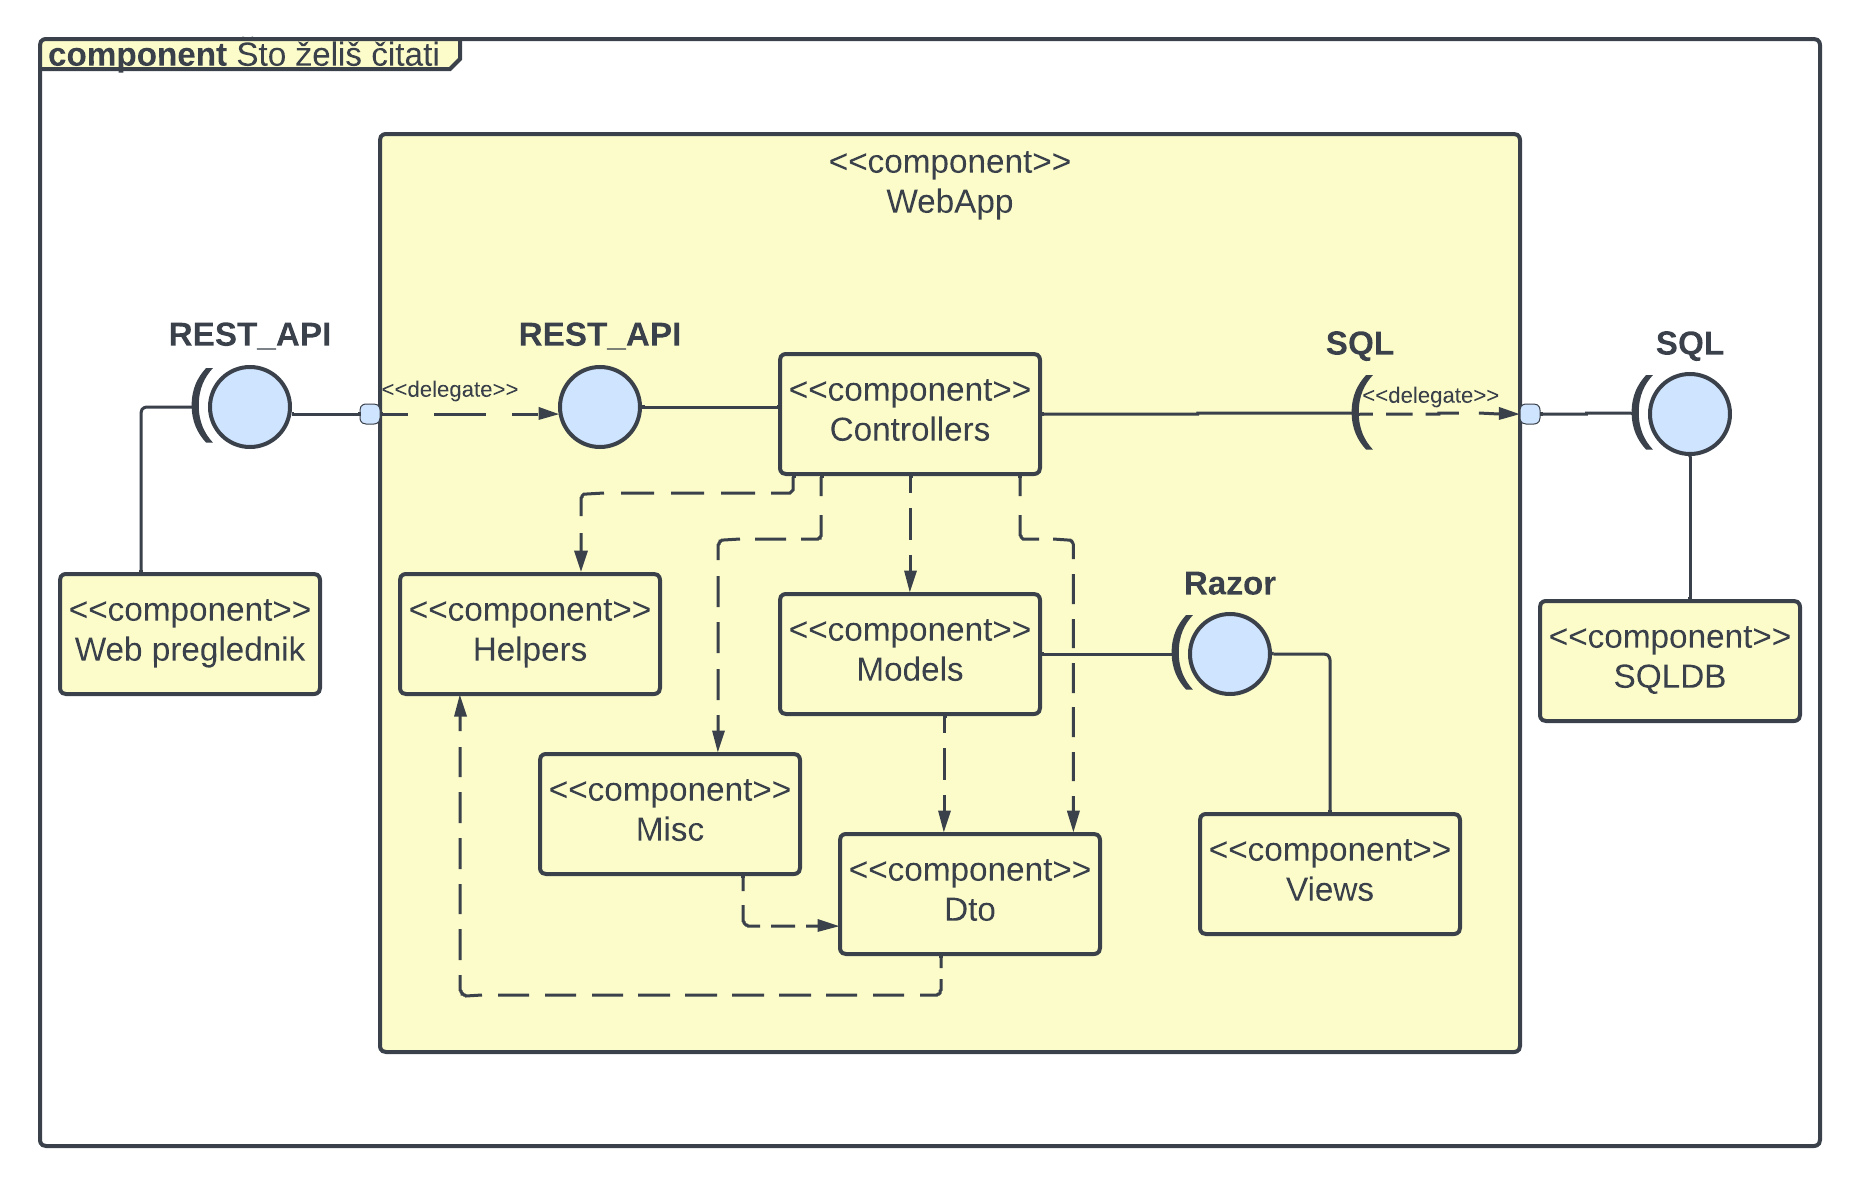
\includegraphics[width = \textwidth]{slike/dijagram_komp.PNG}
				\caption{Dijagram komponenti}
				\label{fig:enter-label}
			\end{figure}
			\eject
			